\svnidlong
{$HeadURL: $}
{$LastChangedDate: $}
{$LastChangedRevision: $}
{$LastChangedBy: $}

\odachapter{\oda black box wrapper cookbook}

\begin{tabular}{p{4cm}l}
\textbf{Contributed by:} & Nils van Velzen\\
\textbf{Last update:}    & \svnfilemonth-\svnfileyear\\
\end{tabular}

\section{What not to expect from this chapter}
This chapter is not a thorough reference manual on configuring and using the
black box wrapper of \oda. The purpose of this chapter is to give you some
overview information to get you started making your own black box wrapper for
your model. There are many example implementations available and at some point
we hope that there will be an user guide available for the black box wrapper
explaining all the details on configuration and implementation. This kind of
detailed information is not to be found in this chapter. This chapter should be
used in combination with the existing examples and the \oda course\footnote{The
  \oda course is available as a separate download from the \oda website.} where
you already can find a lot of information on the black box wrapper.

\section{The design of the black box wrapper}
Using models in black box form in \oda means that data assimilation and model
calibration techniques are applied to a model without changing the existing
model code. \oda and the black box wrapper have no knowledge of the model
internals (black box) and only uses the input and output files of the model.
The black box implementation of \oda can also be used in a slightly different
way as well like we do for C\# models and EFDC, but this is beyond the scope of
this document.


The black box wrapper is an implementation of a stochastic model in \oda. The
difference with a normal model is that the black box wrapper does not contain
any model equations. It is a layer that helps you to link and configure a model
to \oda using the black box approach. The black box wrapper is illustrated in
Figure \ref{Fig:overview}, the elements of this figure will be explained in
some more detail in the following sections.


\begin{figure}[h]
\begin{center}
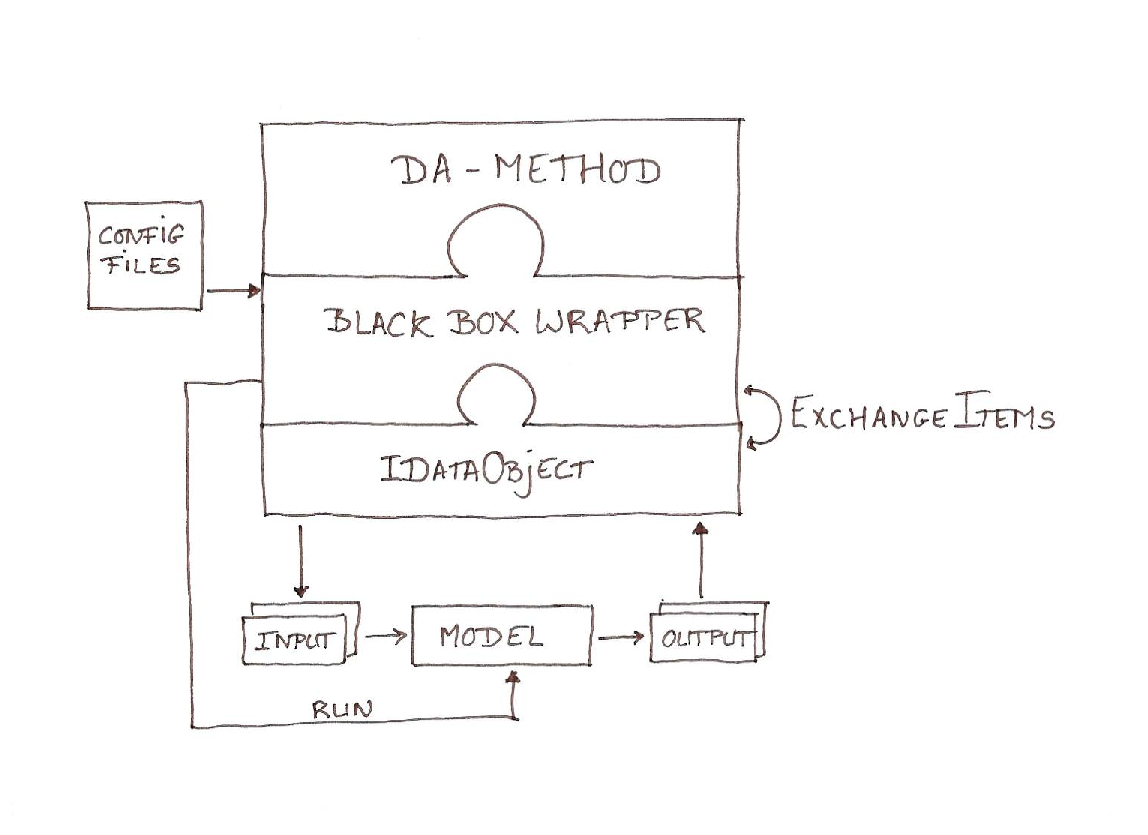
\includegraphics[scale=0.7]{./blackbox/bb_overview.pdf}
\caption{Overview of a black box configuration in \oda. The model interacts
  with the generic black box wrapper of \oda implementing an \oda stochastic
  model. The black box wrapper builds its state, parameters and predictions
  using exchangeItems. The exchangeItems contain values that are read from
  model output files or need to be written to model input files. The creation
  of the exchangeItems and reading from/writing to files is implemented by one
  or more IDataObjects. The black box wrapper will run the model executable when
  all input files are prepared.}
\label{Fig:overview}
\end{center}
\end{figure}


\section{ExchangeItems}
Values from the input and output files are represented in the \oda black box
wrapper in the form of exchangeItems. An exchangeItem is a container of values
with optionally some meta information. In the most simple form an exchangeItem
contains a single value or array and has en ID. ExchangeItems can have three
different roles:
\begin{itemize}
\item input: the values have been read from one of the output files of the
  model. These values are used by the algorithm but (updated) values will not
  be written back to the file.
\item output: the values will be computed by the algorithm and will be written
  to the input file of the model.
\item inout: the values are both read and written to a file of the model that
  is both input as output (typically restart files).
\end{itemize}

There is one special kind of exchangeItem that is now worth mentioning and that
is the timeSeriesExchangeItem. This kind of exchangeItem contains a sequence of
values that are all associated to a timestamp (meta information). This kind of
exchangeItem is typically used for storing model results that need to be
matched to observations.

\section{Model wrappers}
The model uses files for input and output and the black box wrapper uses
exchangeItems. Therefore we need to write some code that creates all the
exchangeItems and handles the reading and writing of the values in the
exchangeItems from and to the model input and output files.

For each file format we need to handle we have to implement a java class that
implements the IDataObjectInterface interface. This interface only contains three
public methods:
\begin{itemize}
\item initialize: creates all exchangeItems. The values of the input and inout
  exchangeItems are read from file.
\item getExchangeItems: Returns an array containing all the exchangeItems of
  this file.
\item finish: Write the values of output and inout exchangeItems to file.
\end{itemize}

\oda already contains quite a number of implementations of exchangeItems. In
almost all cases you can use one of the existing implementations as container
of the values for your model. Useful existing implementations include:
\begin{itemize}
\item org.openda.exchange.DoubleExchangeItem: ExchangeItem for a single double
\item org.openda.exchange.DoublesExchangeItem: ExchangeItem for an array of
  doubles
\item org.openda.exchange.timeseries.TimeSeries: Timeseries of double values
  each having a time associated.
\end{itemize}

Your implementation only needs to create those exchangeItems that you think you
will need. In an first implementation you do not need to bother about all
possible data in the files. Additional exchangeItems can always be added later
when needed.

\section{Recipe}
\begin{itemize}
\item Identify the input and output files that contain values you need and
  determine how these values are stored
\item Write an IDataObjectInterface class for each file format you need such that
  you have exchangeItems for all the data you are going to use in \oda. Try to
  use existing implementations of exchangeItems when possible. For inspiration
  look at available example implementations. Note: Use a "simple" wrapper like
  reactive\_advection\_pollution\_wrapper from the \oda course or model\_nemo
  as inspiration and not one of the very complex wrappers with a lot of support
  and functionality.
\item set up a black box configuration environment (model input and
  configuration files). Best way is to copy an existing example and replace
  model input files and change the black box configuration files. The basic
  ideas of the black box configuration are explained in the \oda course.
\item Done
\end{itemize}





